\chapter{Training Curves}\label{app:curves}


%%%%%%%%%%%%%%%%%%%%%%%%%%%%%%%%%%%%%%%%%%%%%%%%%%%%%%%

\section{Benchmark classifier}\label{curves:benchmark}

\begin{figure}[htbp]
    \centering
    \begin{subfigure}[htbp]{\textwidth}
        \centering
        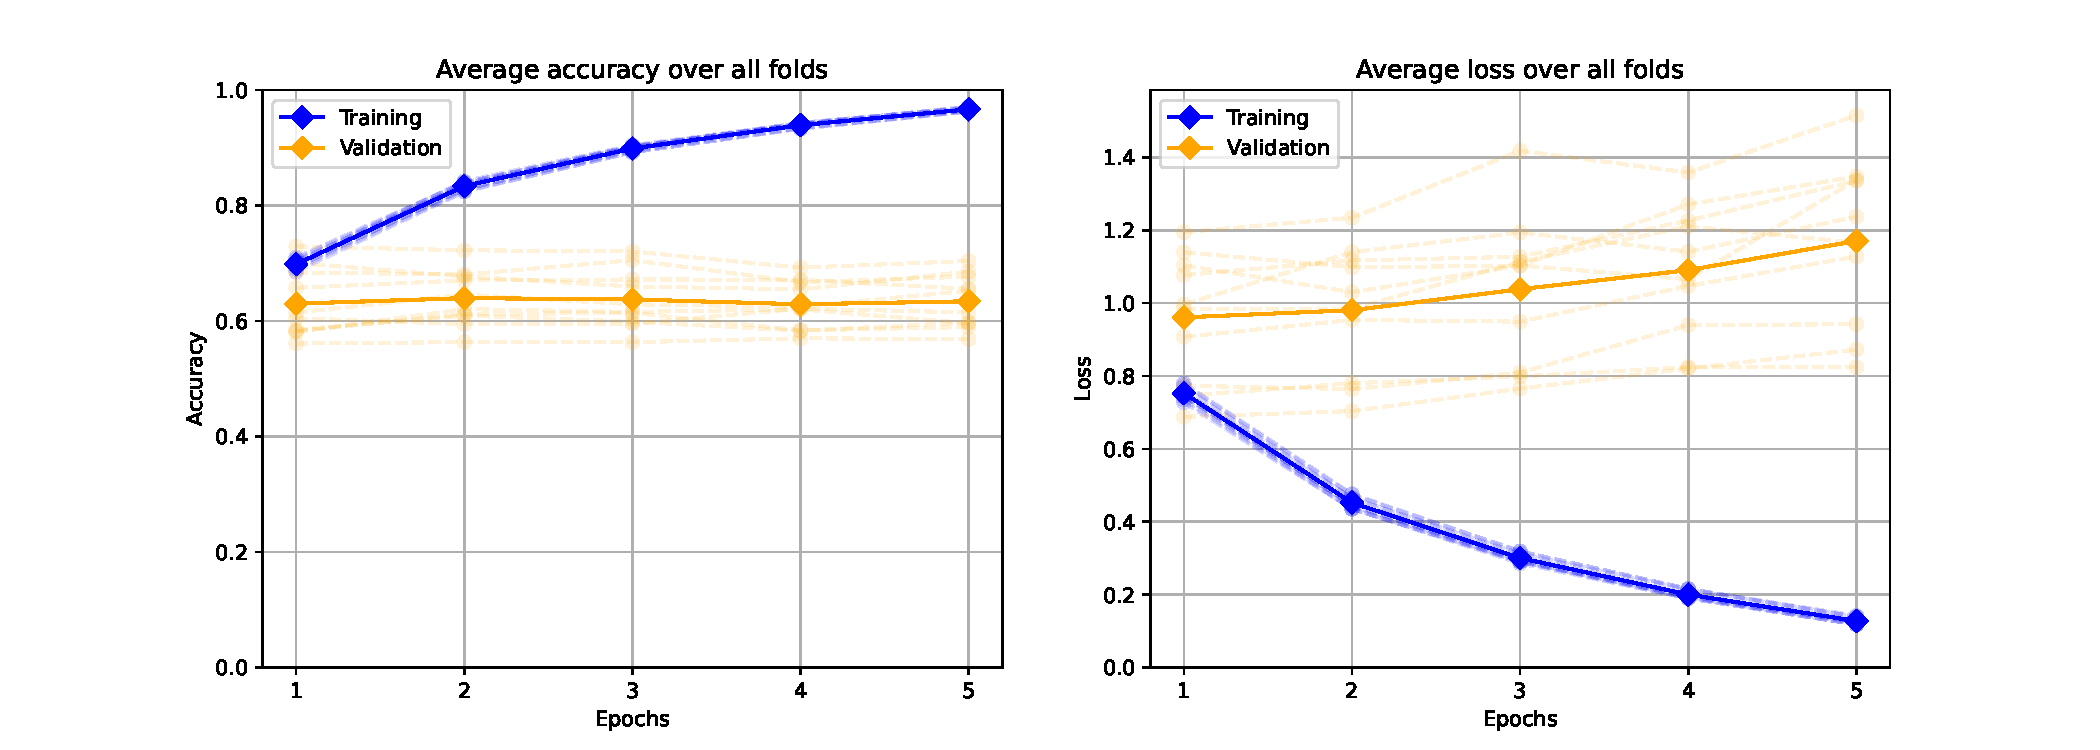
\includegraphics[trim={3cm 0 3cm 0.8cm},clip,width=\textwidth]{img/ch3/baseline_results/cnn_lstm_by_epoch.pdf}
        \caption{Accuracy and loss curves across all folds by epoch.}
        \label{fig:baseline-by-epoch}
    \end{subfigure}
    
    \vspace{0.5cm}
    
    \begin{subfigure}[htbp]{\textwidth}
        \centering
        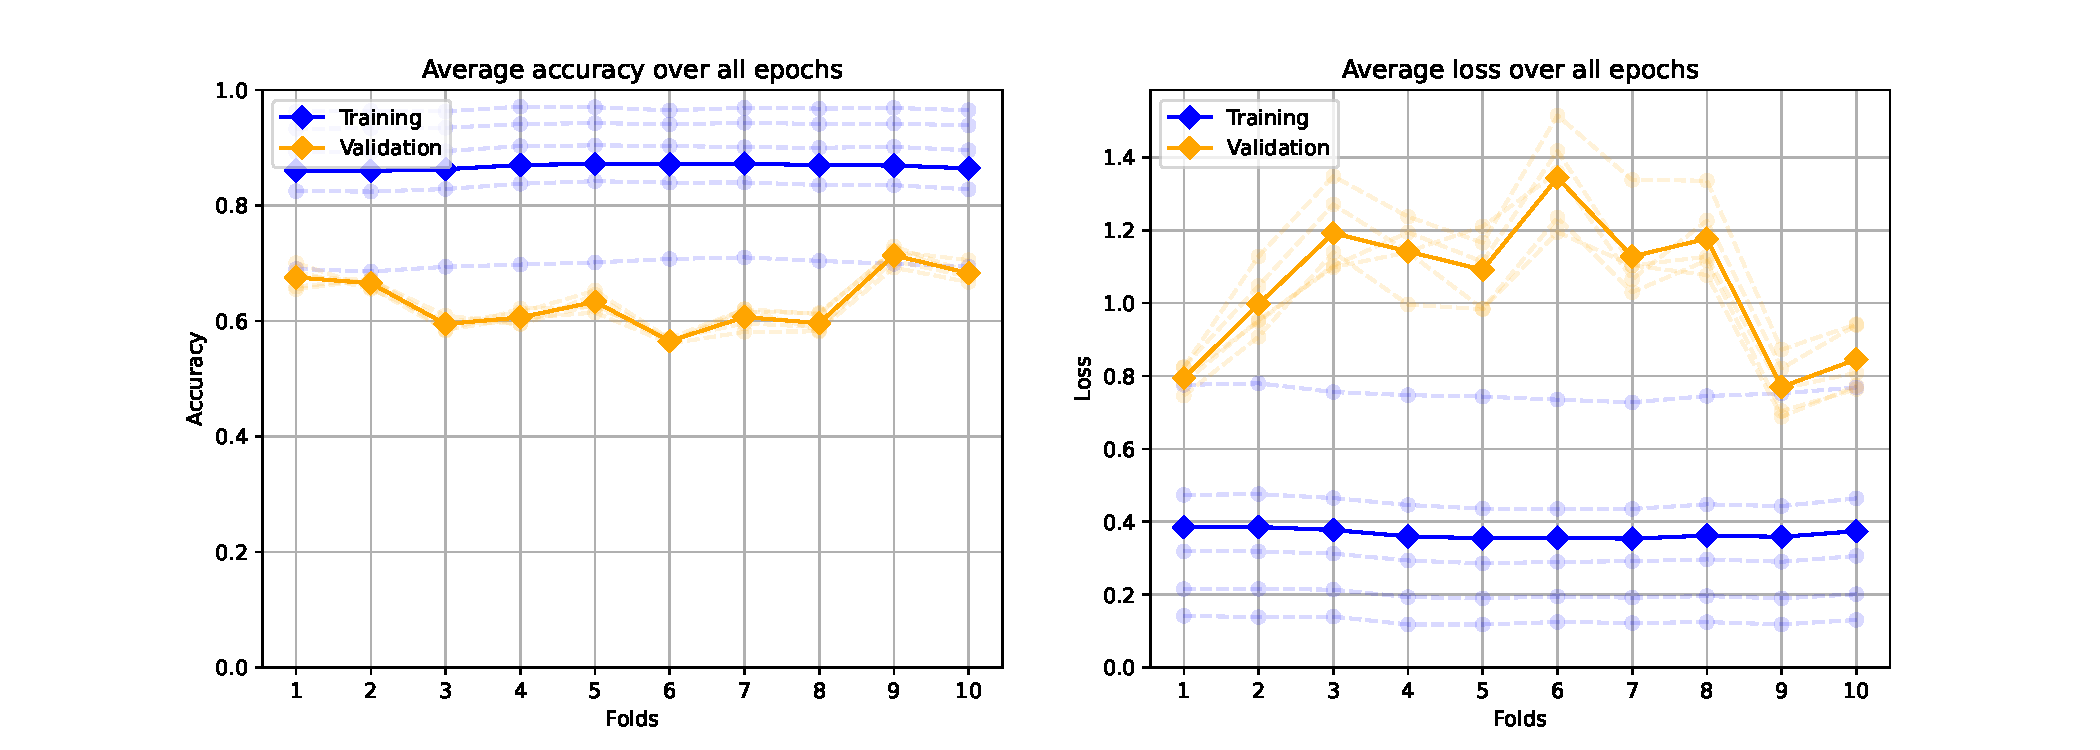
\includegraphics[trim={3cm 0 3cm 0.8cm},clip,width=\textwidth]{img/ch3/baseline_results/cnn_lstm_by_fold.pdf}
        \caption{Accuracy and loss curves across all epochs by fold.}
        \label{fig:baseline-by-fold}
    \end{subfigure}
    \caption{Training and validation accuracy and loss curves for the benchmark CNN-LSTM model.}
    \label{fig:baseline-acc-loss}
\end{figure}


%%%%%%%%%%%%%%%%%%%%%%%%%%%%%%%%%%%%%%%%%%%%%%%%%%%%%%5

\newpage
\section{Normalisation experiments}\label{curves:normalisation}
\vfill
\begin{figure}[htbp]
    \centering
    \begin{subfigure}{\textwidth}
        \centering
        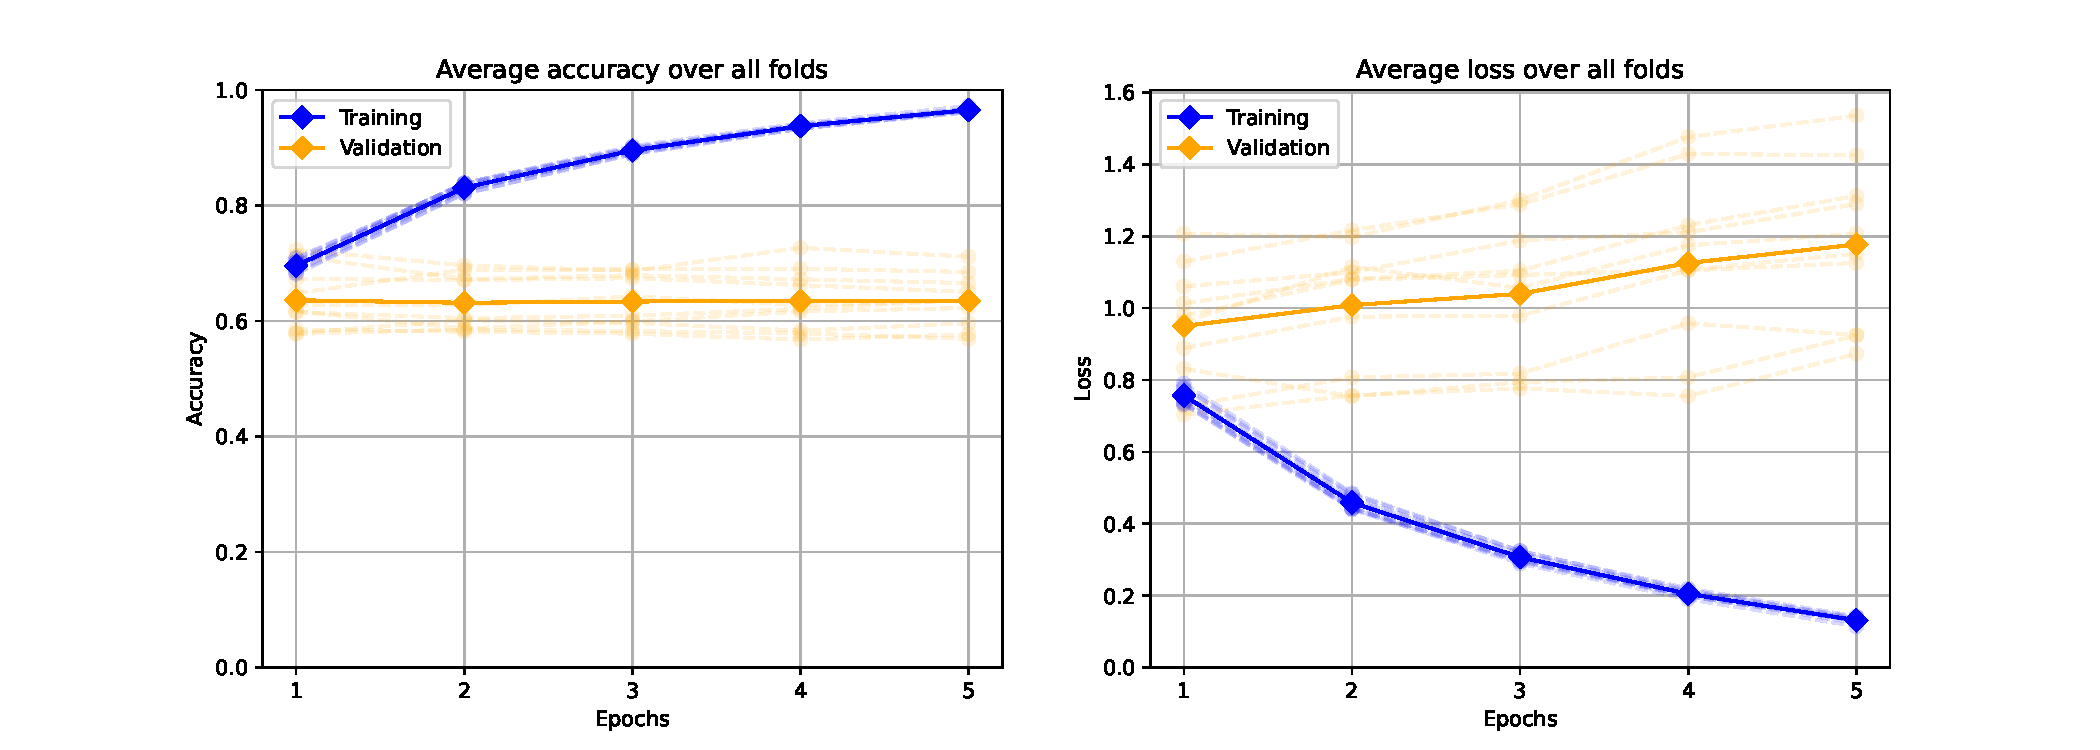
\includegraphics[trim={3cm 0 3cm 0.8cm},clip,width=\textwidth]{img/ch4/channel/channel_by_epoch.pdf}
        \caption{Training and validation accuracy and loss trends per epoch for the channel normalisation experiment.}
        \label{channel-norm-by-epoch}
    \end{subfigure}
    
    \vspace{1cm}
    
    \begin{subfigure}{\textwidth}
        \centering
        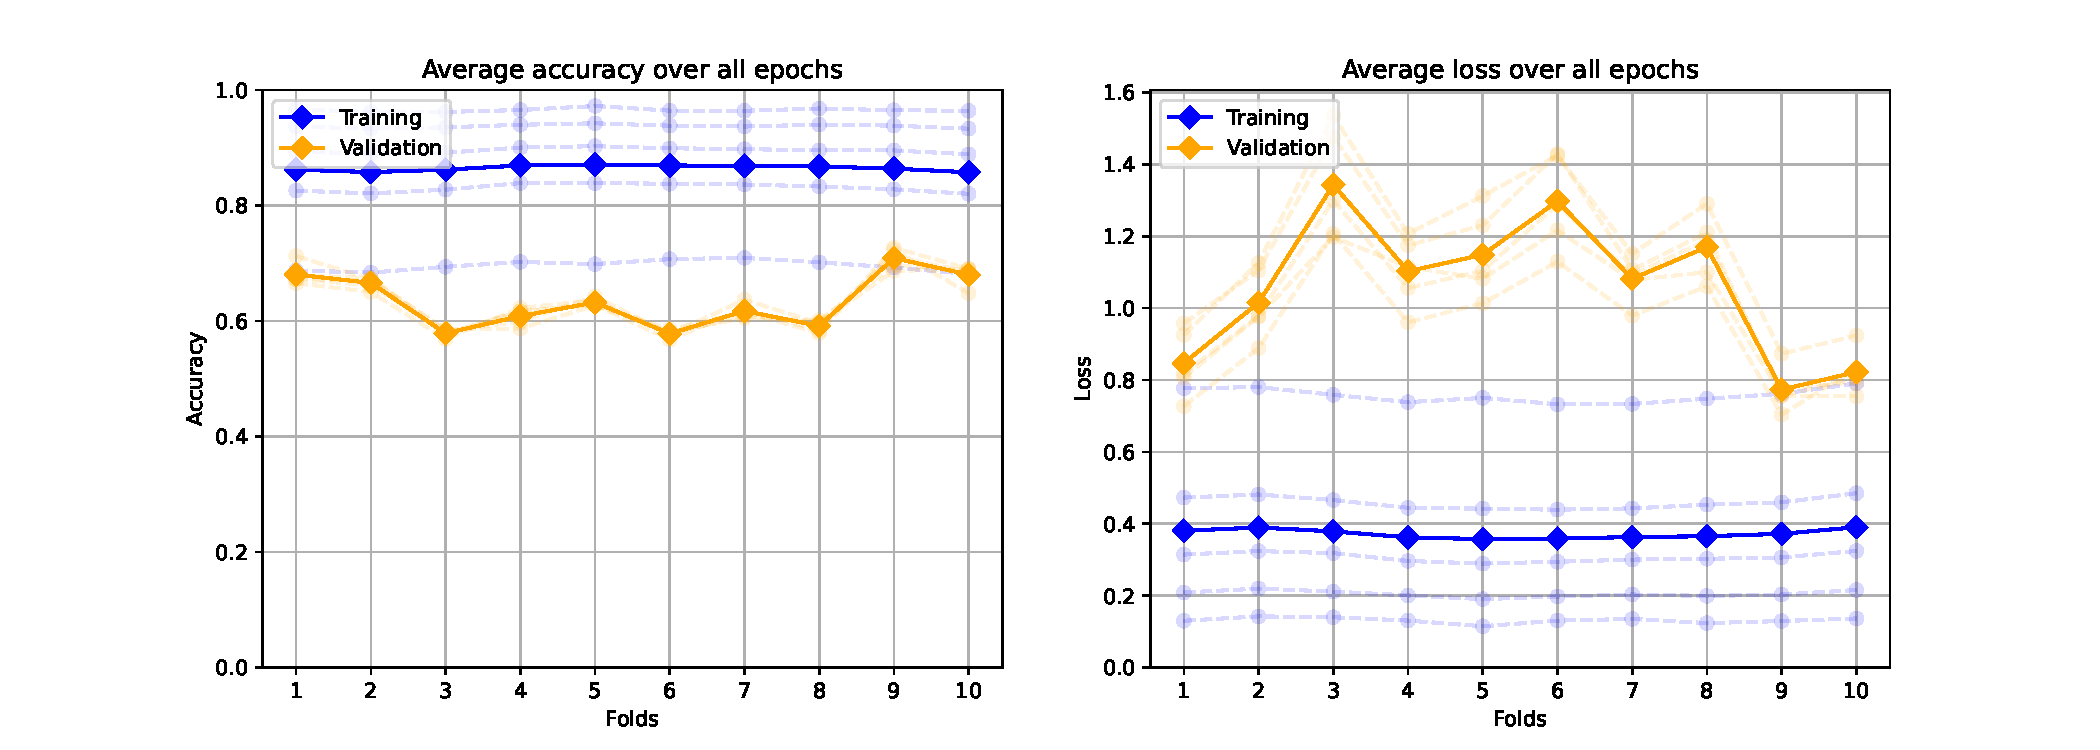
\includegraphics[trim={3cm 0 3cm 0.8cm},clip,width=\textwidth]{img/ch4/channel/channel_by_fold.pdf}
        \caption{Training and validation accuracy and loss trends per fold for the channel normalisation experiment.}
        \label{fig:channel-norm-by-fold}
    \end{subfigure}
    \caption{Comparison of training and validation performance for channel normalisation, showing accuracy and loss curves evaluated by (a) epoch and (b) fold.} 
    \label{fig:channel-norm-acc-loss}
\end{figure}
\vfill
\begin{figure}[htbp]
    \centering
    \begin{subfigure}{\textwidth}
        \centering
        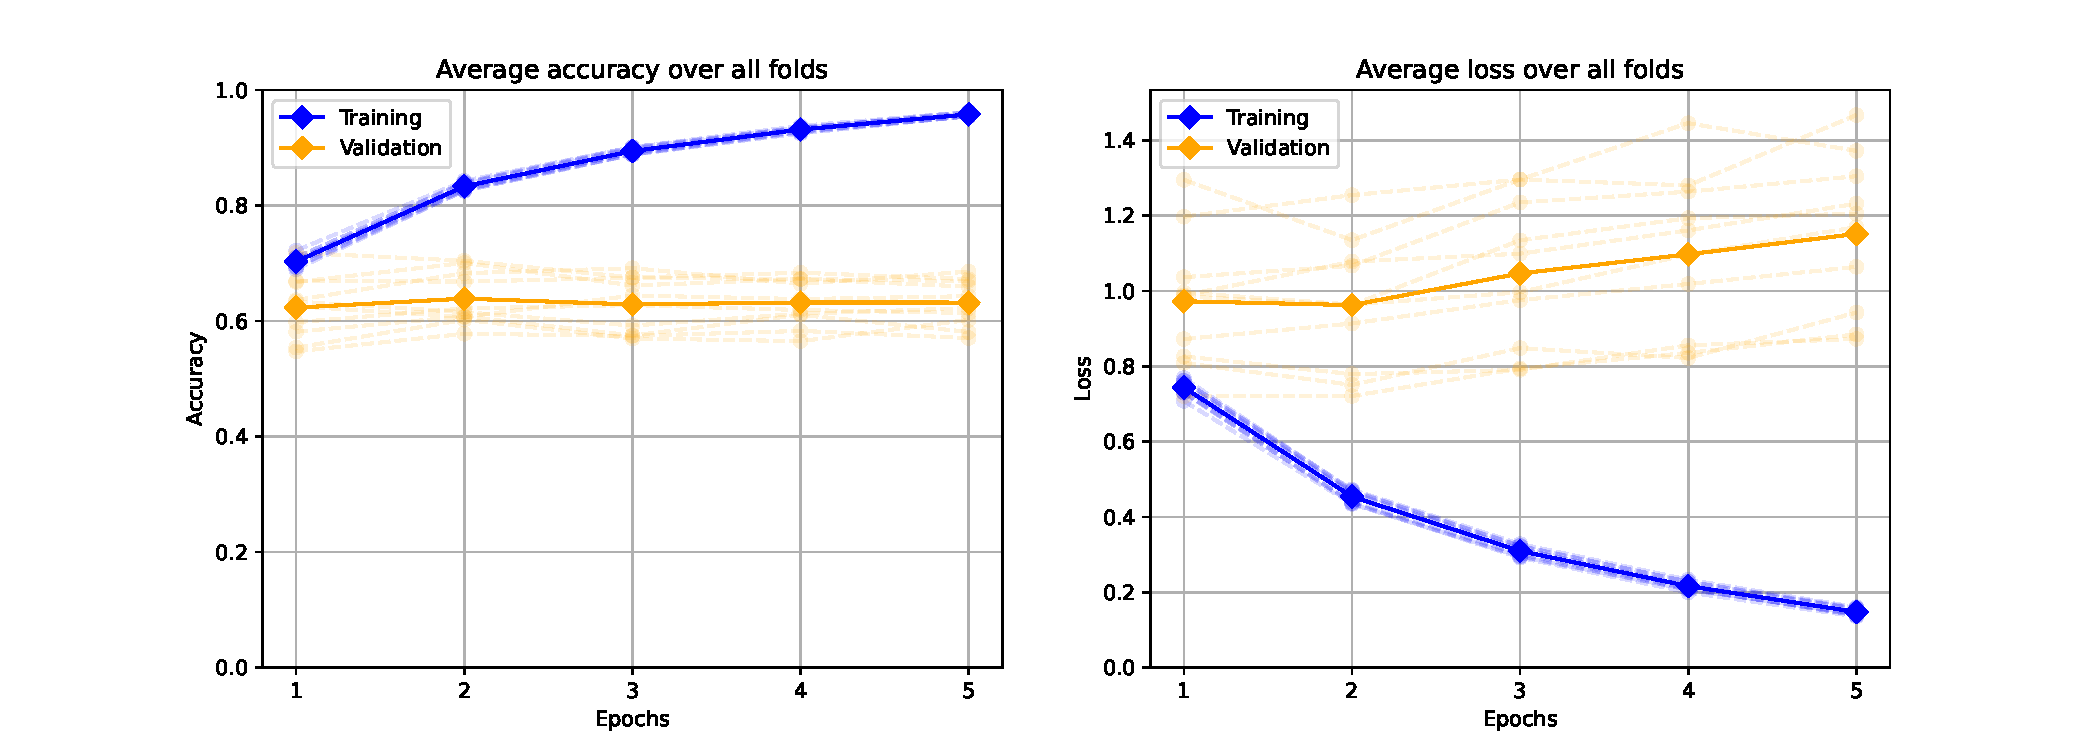
\includegraphics[trim={3cm 0 3cm 0.8cm},clip,width=\textwidth]{img/ch4/global/global_by_epoch.pdf}
        \caption{Training and validation accuracy and loss trends per epoch for the global normalisation experiment.}
        \label{global-norm-by-epoch}
    \end{subfigure}
    
    \vspace{1cm}
    
    \begin{subfigure}{\textwidth}
        \centering
        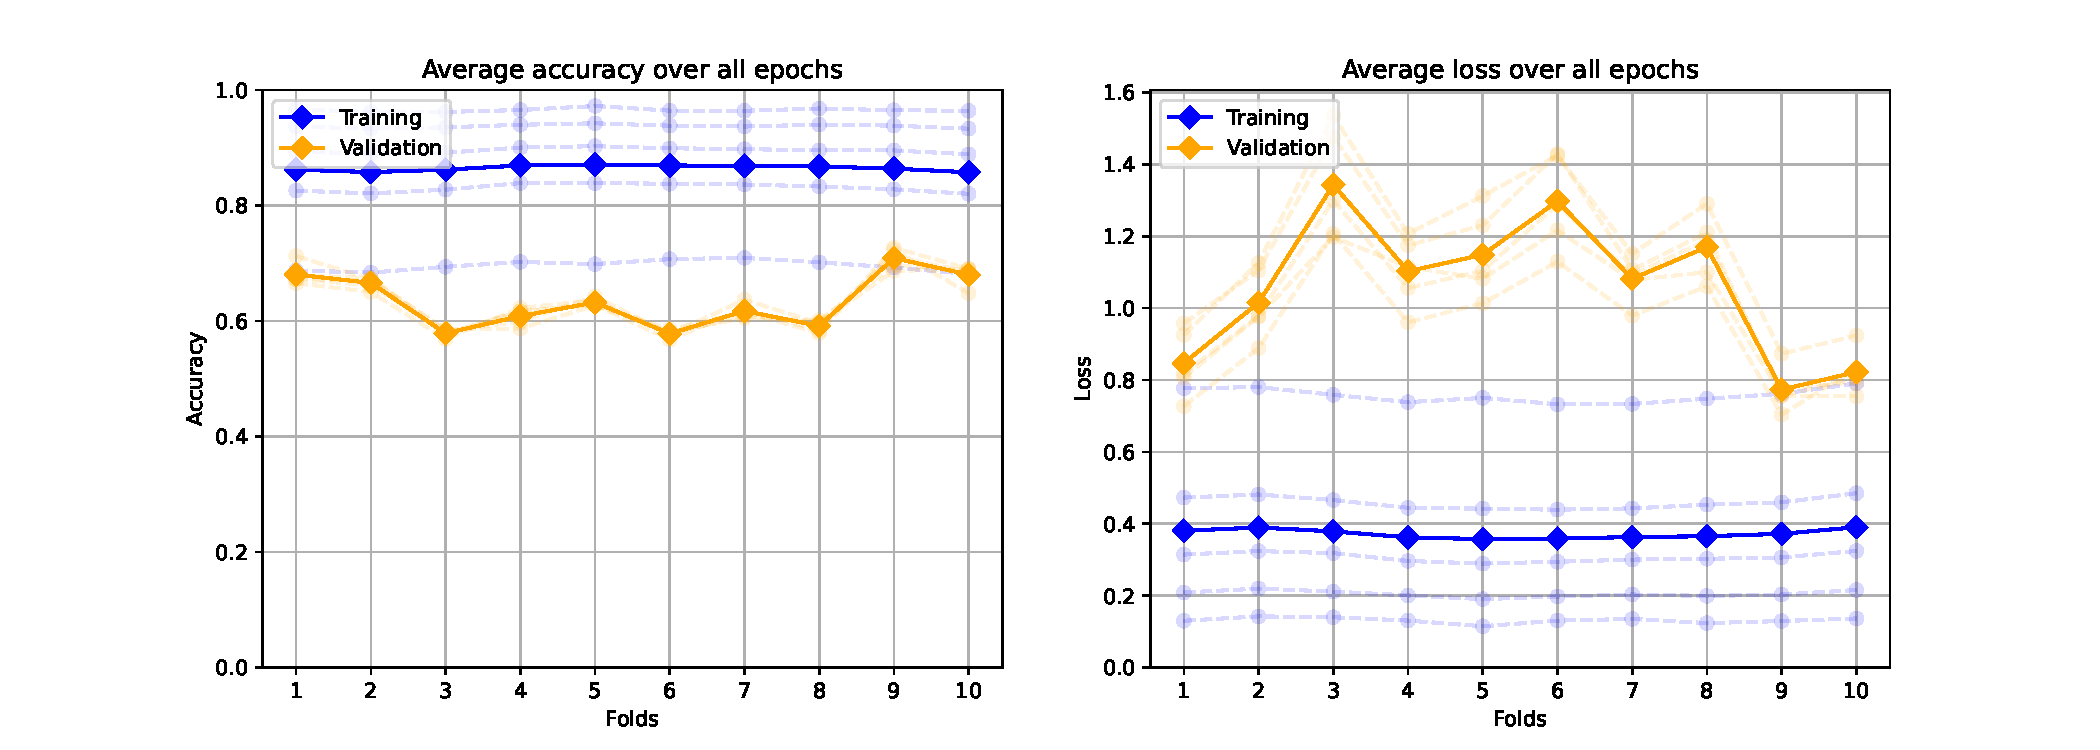
\includegraphics[trim={3cm 0 3cm 0.8cm},clip,width=\textwidth]{img/ch4/channel/channel_by_fold.pdf}
        \caption{Training and validation accuracy and loss trends per fold for the global normalisation experiment.}
        \label{fig:global-norm-by-fold}
    \end{subfigure}
    \caption{Comparison of training and validation performance for global normalisation, showing accuracy and loss curves evaluated by (a) epoch and (b) fold.} 
    \label{fig:global-norm-acc-loss}
\end{figure}

%%%%%%%%%%%%%%%%%%%%%%%%%%%%%%%%%%%%%%%%%%%%%%%%%%%%%%%%

\newpage
\section{Detrending experiments}\label{curves:detrending}

\begin{figure}[htbp]
    \centering
    \begin{subfigure}{\textwidth}
        \centering
        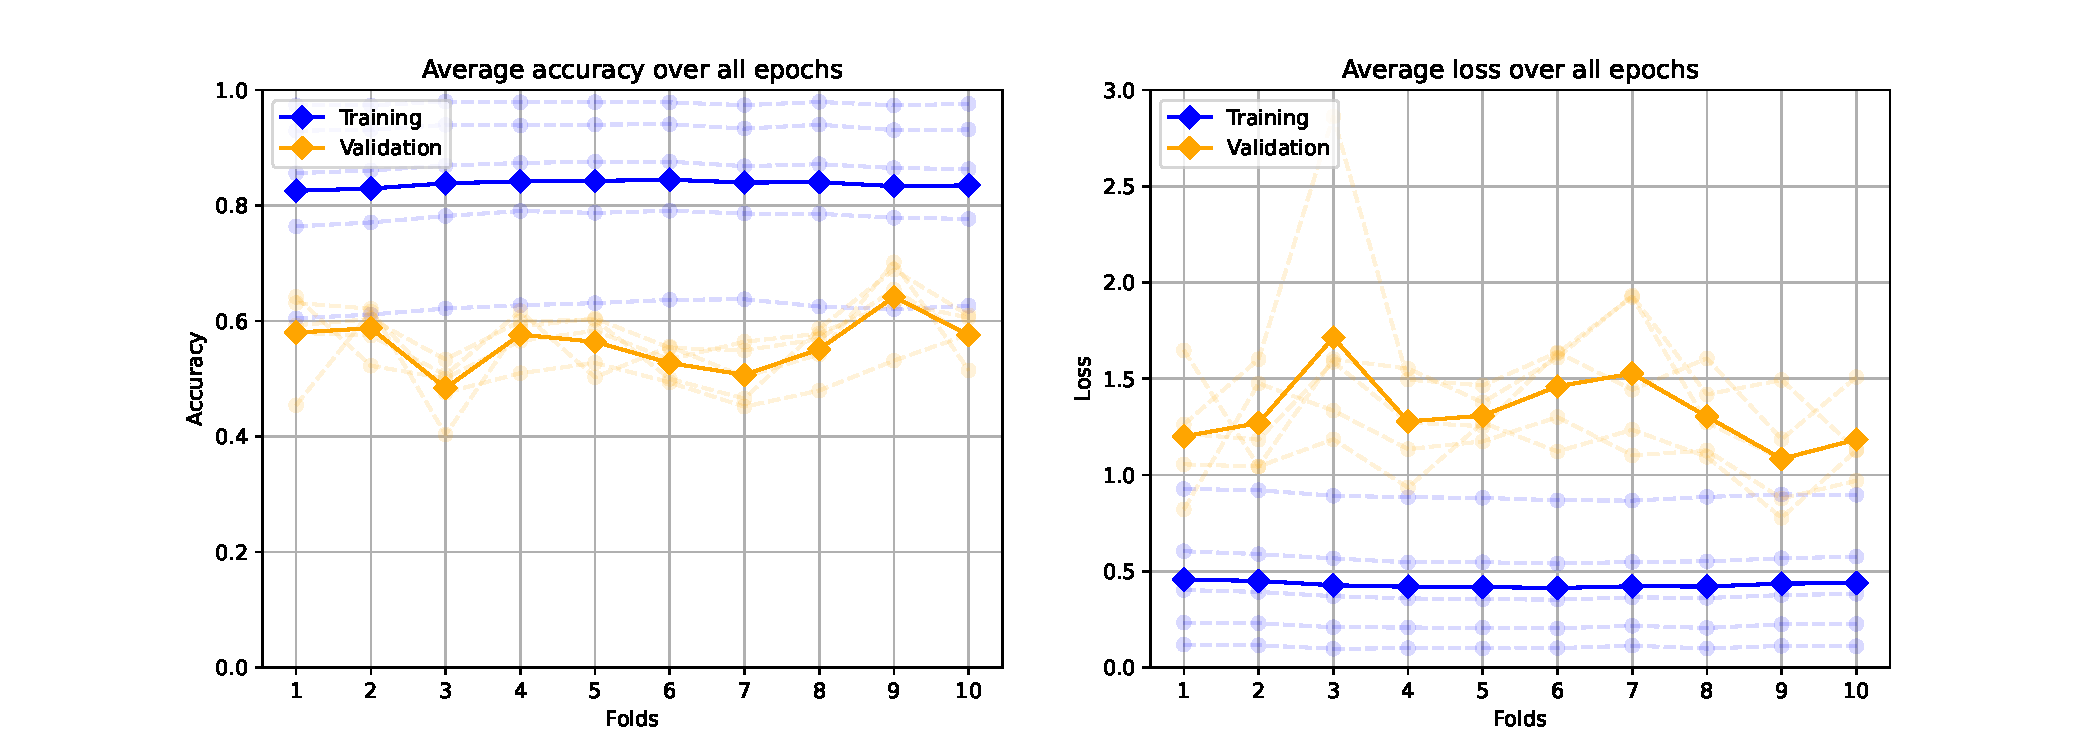
\includegraphics[trim={3cm 0 3cm 0.8cm},clip,width=\textwidth]{img/ch5/e0_3_epochs_by_fold.pdf}
        \caption{Validation accuracy and loss by fold for $\ell_1$ detrending with $\alpha = 1$.}
        \label{fig:detrend-acc-loss-e0-fold}
    \end{subfigure}

    \vspace{0.5cm}
    
    \begin{subfigure}{\textwidth}
        \centering
        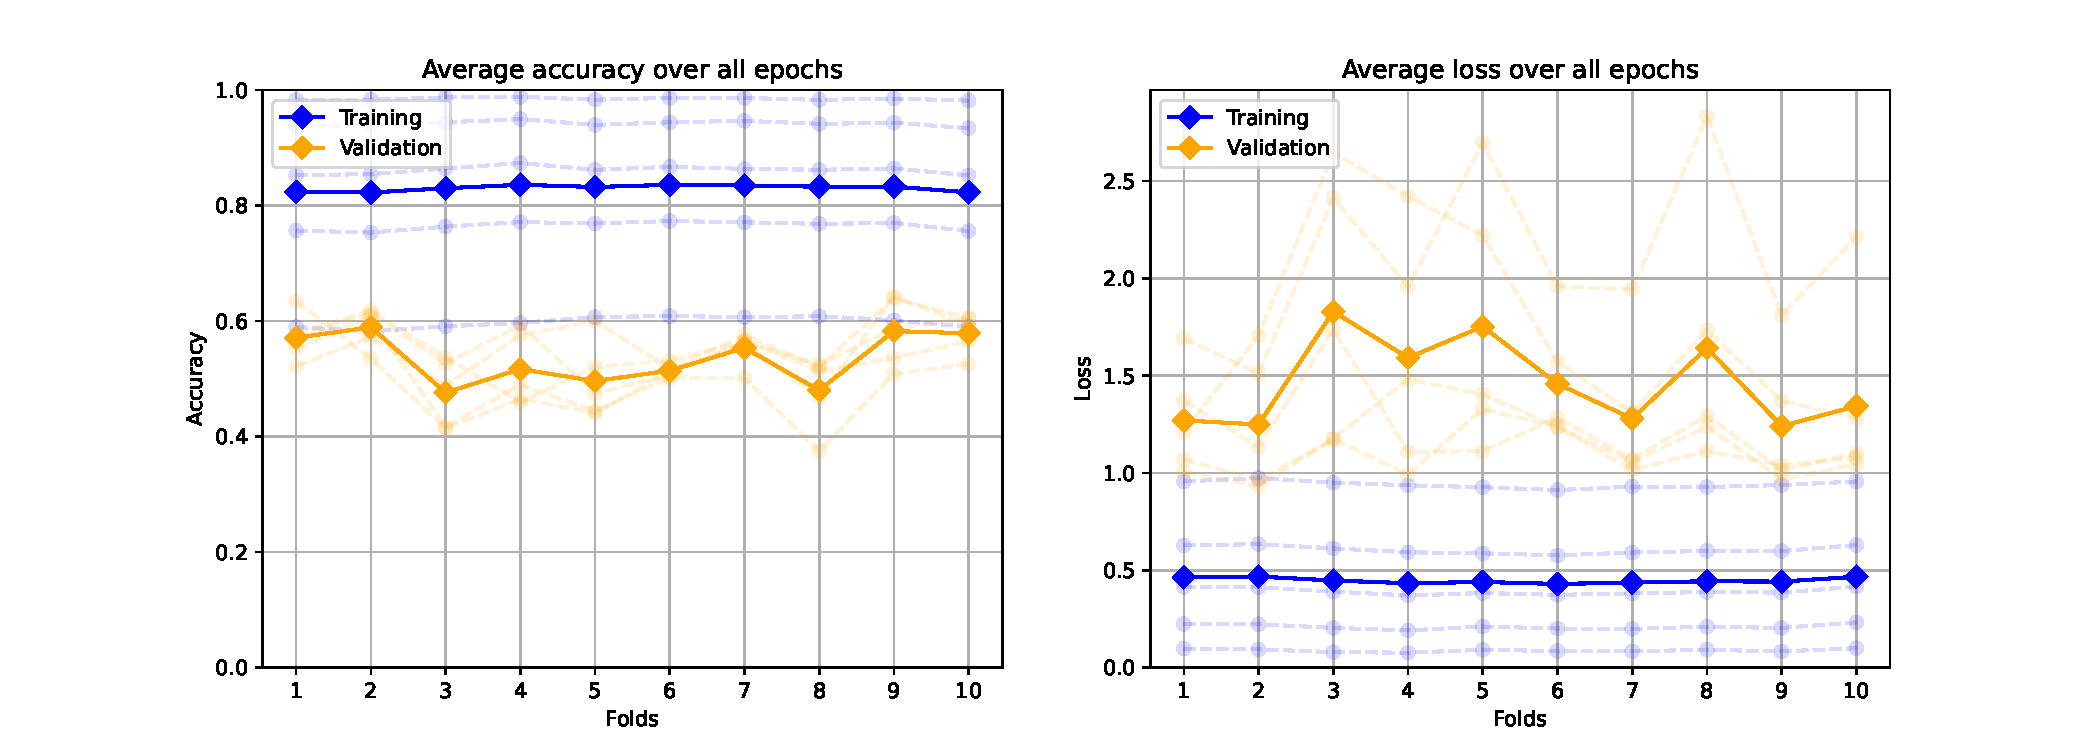
\includegraphics[trim={3cm 0 3cm 0.8cm},clip,width=\textwidth]{img/ch5/e-1_3_epochs_by_fold.pdf}
        \caption{Validation accuracy and loss by fold for $\ell_1$ detrending with $\alpha = 10^{-1}$.}
        \label{fig:detrend-acc-loss-e-1-fold}
    \end{subfigure}

    \vspace{0.5cm}
    
    \begin{subfigure}{\textwidth}
        \centering
        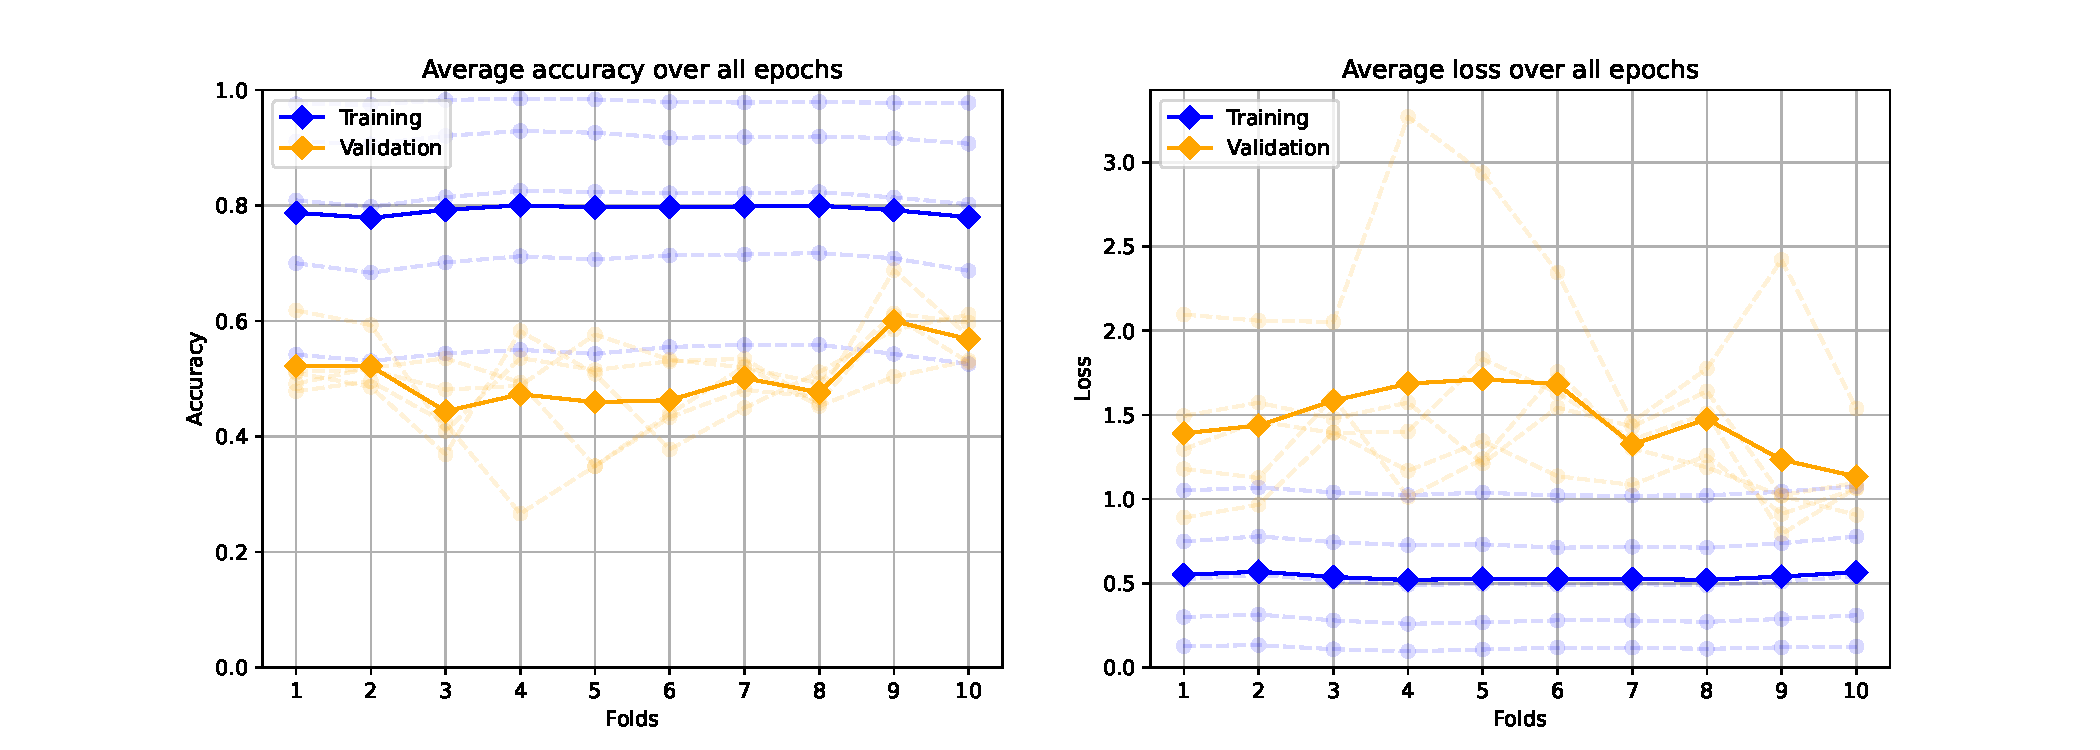
\includegraphics[trim={3cm 0 3cm 0.8cm},clip,width=\textwidth]{img/ch5/e-2_3_epochs_by_fold.pdf}
        \caption{Validation accuracy and loss by fold for $\ell_1$ detrending with $\alpha = 10^{-2}$.}
        \label{fig:detrend-acc-loss-e-2-fold}
    \end{subfigure}
    \caption{Validation accuracy and loss curves for $\ell_1$ detrending experiments by fold. Faint lines show curves for individual epochs while the dark line shows the average across all epochs.} 
    \label{fig:detrend-acc-loss-curves-fold}
\end{figure}

\begin{figure}[p]
    \centering
    \begin{subfigure}{\textwidth}
        \centering
        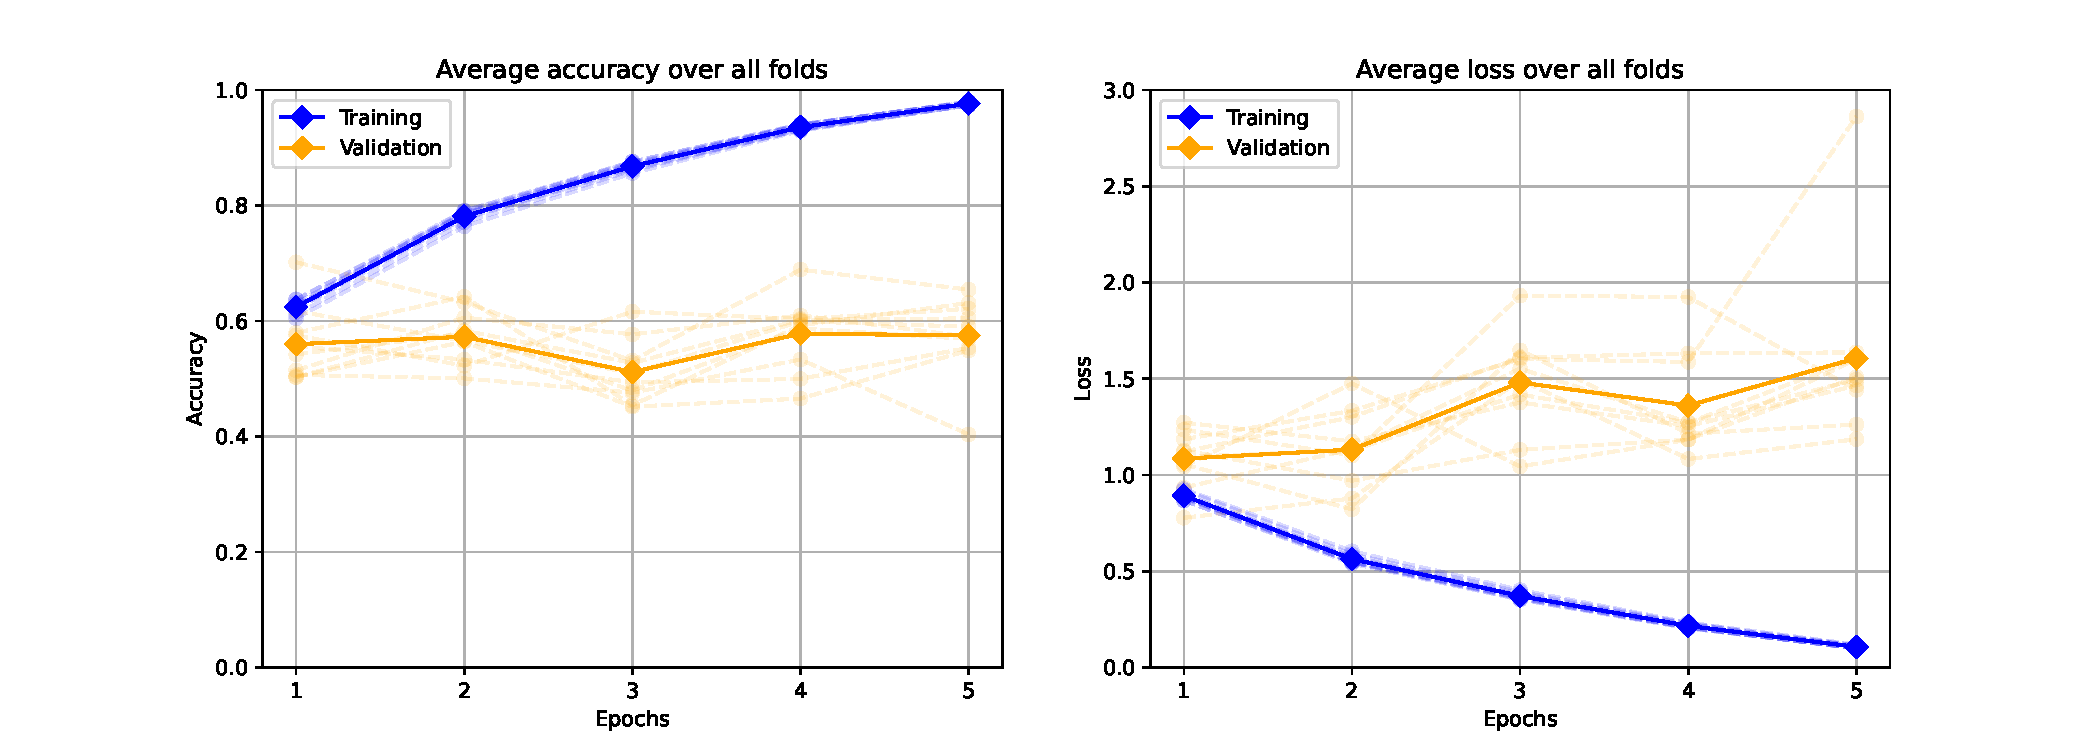
\includegraphics[trim={3cm 0 3cm 0.8cm},clip,width=\textwidth]{img/ch5/e0_3_epochs_by_epoch.pdf}
        \caption{Validation accuracy and loss by epoch for $\ell_1$ detrending with $\alpha = 1$.}
        \label{fig:detrend-acc-loss-e0-epoch}
    \end{subfigure}

    \vspace{0.5cm}
    
    \begin{subfigure}{\textwidth}
        \centering
        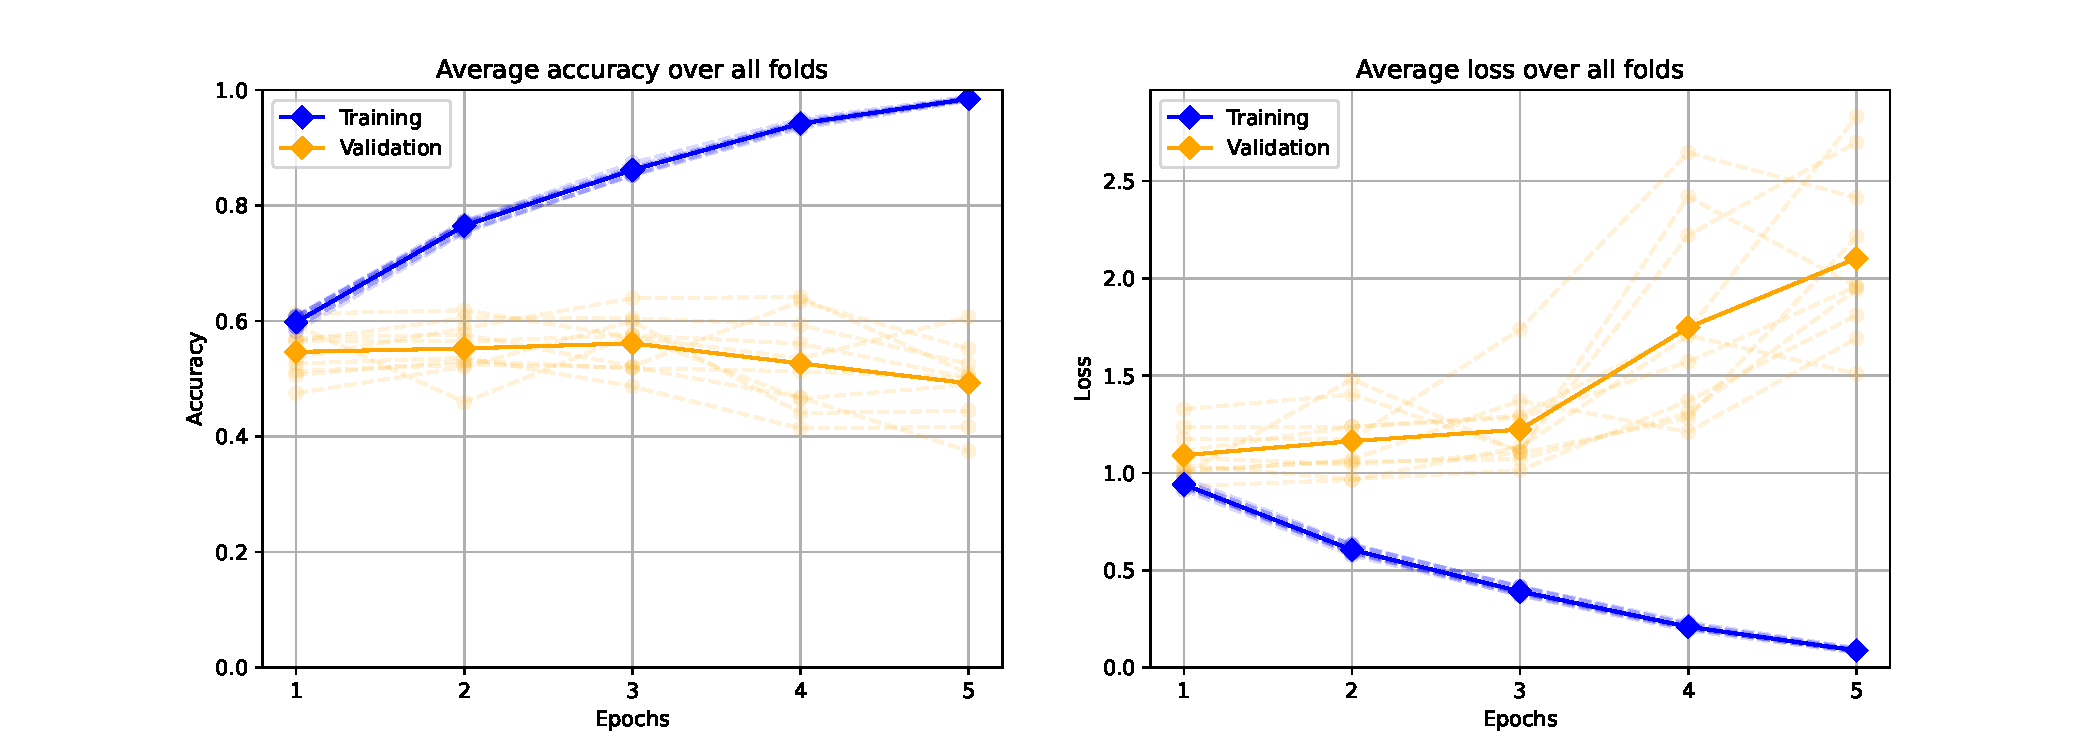
\includegraphics[trim={3cm 0 3cm 0.8cm},clip,width=\textwidth]{img/ch5/e-1_3_epochs_by_epoch.pdf}
        \caption{Validation accuracy and loss by epoch for $\ell_1$ detrending with $\alpha = 10^{-1}$.}
        \label{fig:detrend-acc-loss-e-1-epoch}
    \end{subfigure}

    \vspace{0.5cm}
    
    \begin{subfigure}{\textwidth}
        \centering
        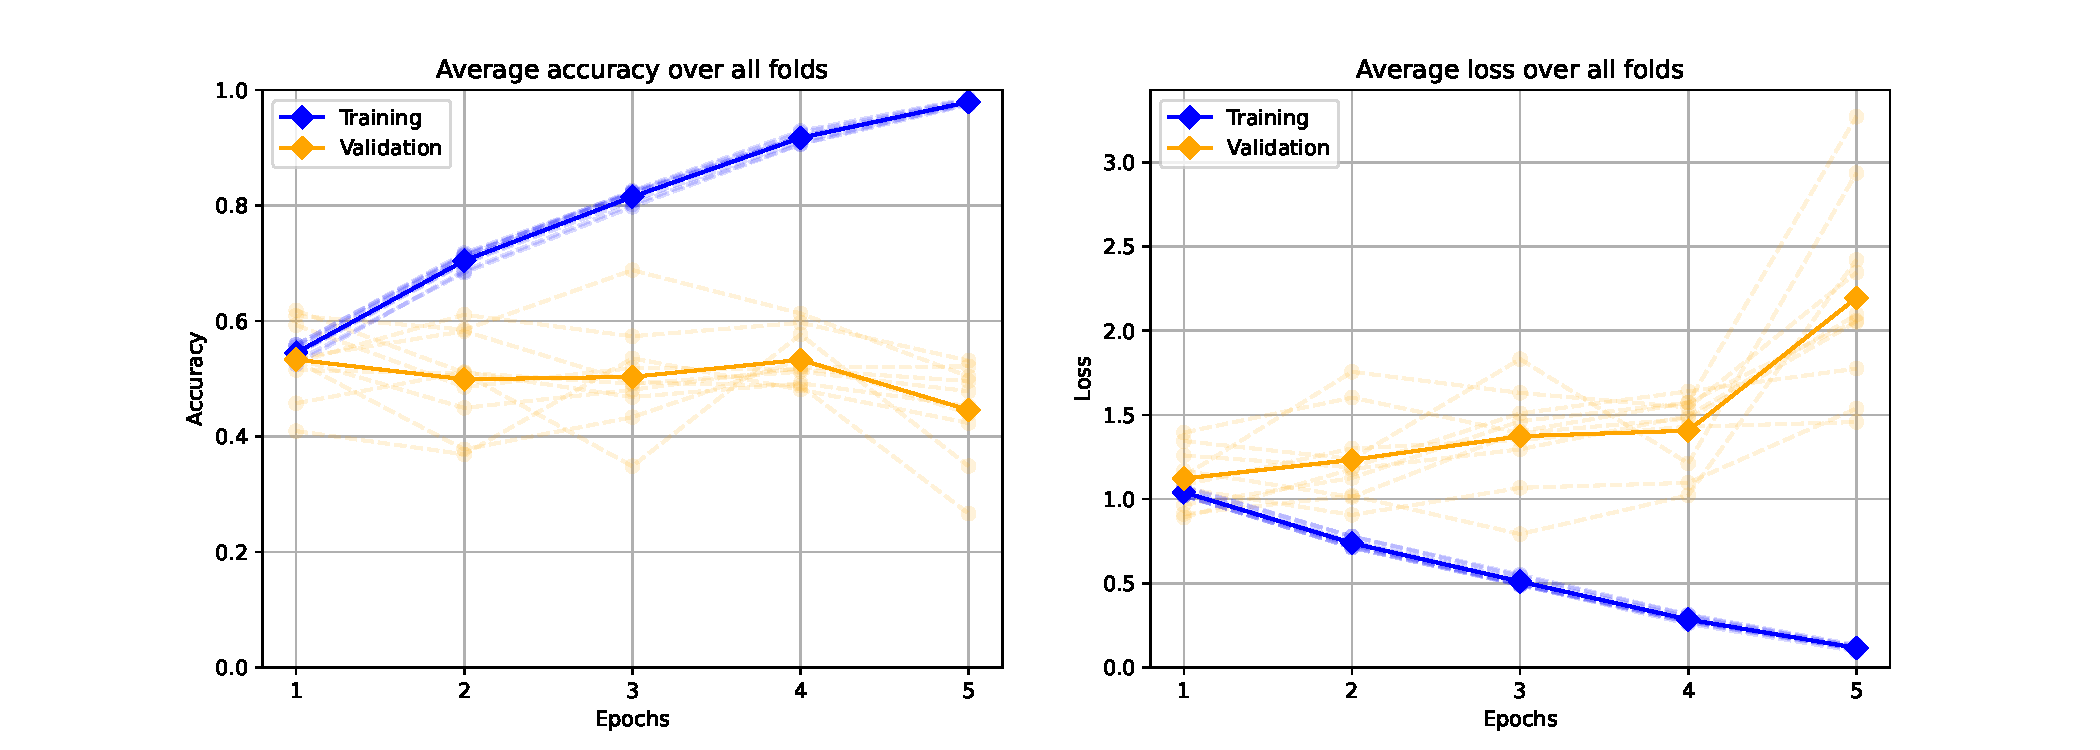
\includegraphics[trim={3cm 0 3cm 0.8cm},clip,width=\textwidth]{img/ch5/e-2_3_epochs_by_epoch.pdf}
        \caption{Validation accuracy and loss by epoch for $\ell_1$ detrending with $\alpha = 10^{-2}$.}
        \label{fig:detrend-acc-loss-e-2-epoch}
    \end{subfigure}
    \caption{Validation accuracy and loss curves for $\ell_1$ detrending experiments by epoch. Faint lines show curves for individual folds while the dark line shows the average across all folds.} 
    \label{fig:detrend-acc-loss-curves-epoch}
\end{figure}

%%%%%%%%%%%%%%%%%%%%%%%%%%%%%%%%%%%%

\newpage
\section{Denoising experiments}

%%%%%
\subsection{Experiment 1}
\begin{figure}[htbp]
    \centering
    \begin{subfigure}{\textwidth}
        \centering
        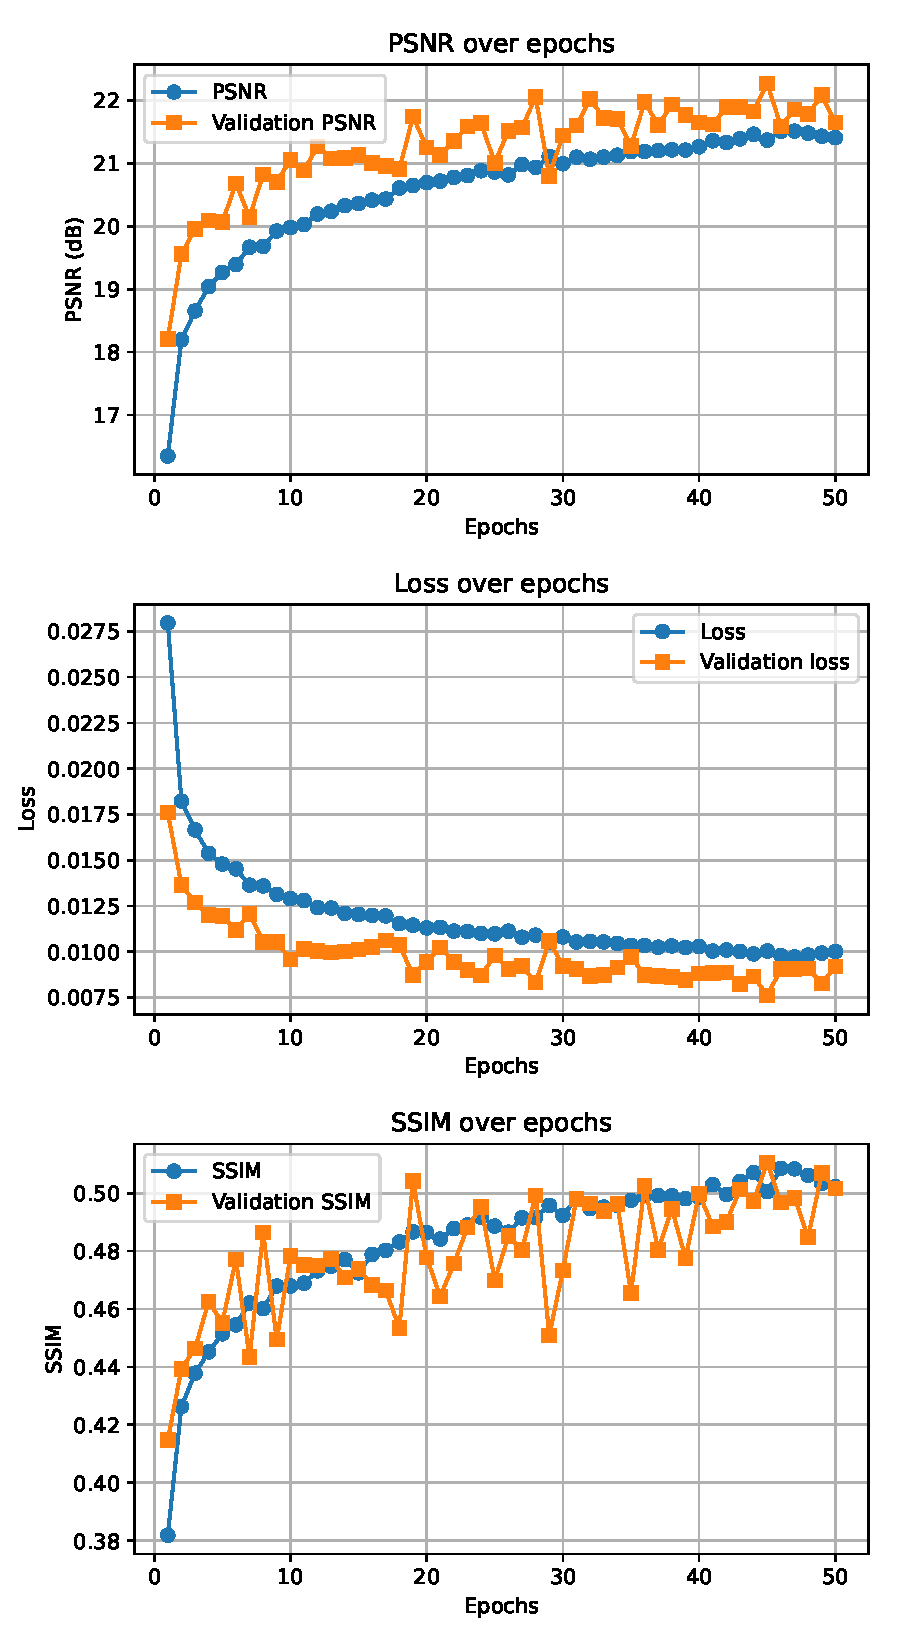
\includegraphics[height=0.9\textheight]{img/ch6/supervised/psnr_loss_irfan.pdf}
        \caption{Irfan}
        \label{fig:denoising-exp1-curves-irfan}
    \end{subfigure}
\end{figure}
\begin{figure}
    \ContinuedFloat
    \begin{subfigure}{\textwidth}
        \centering
        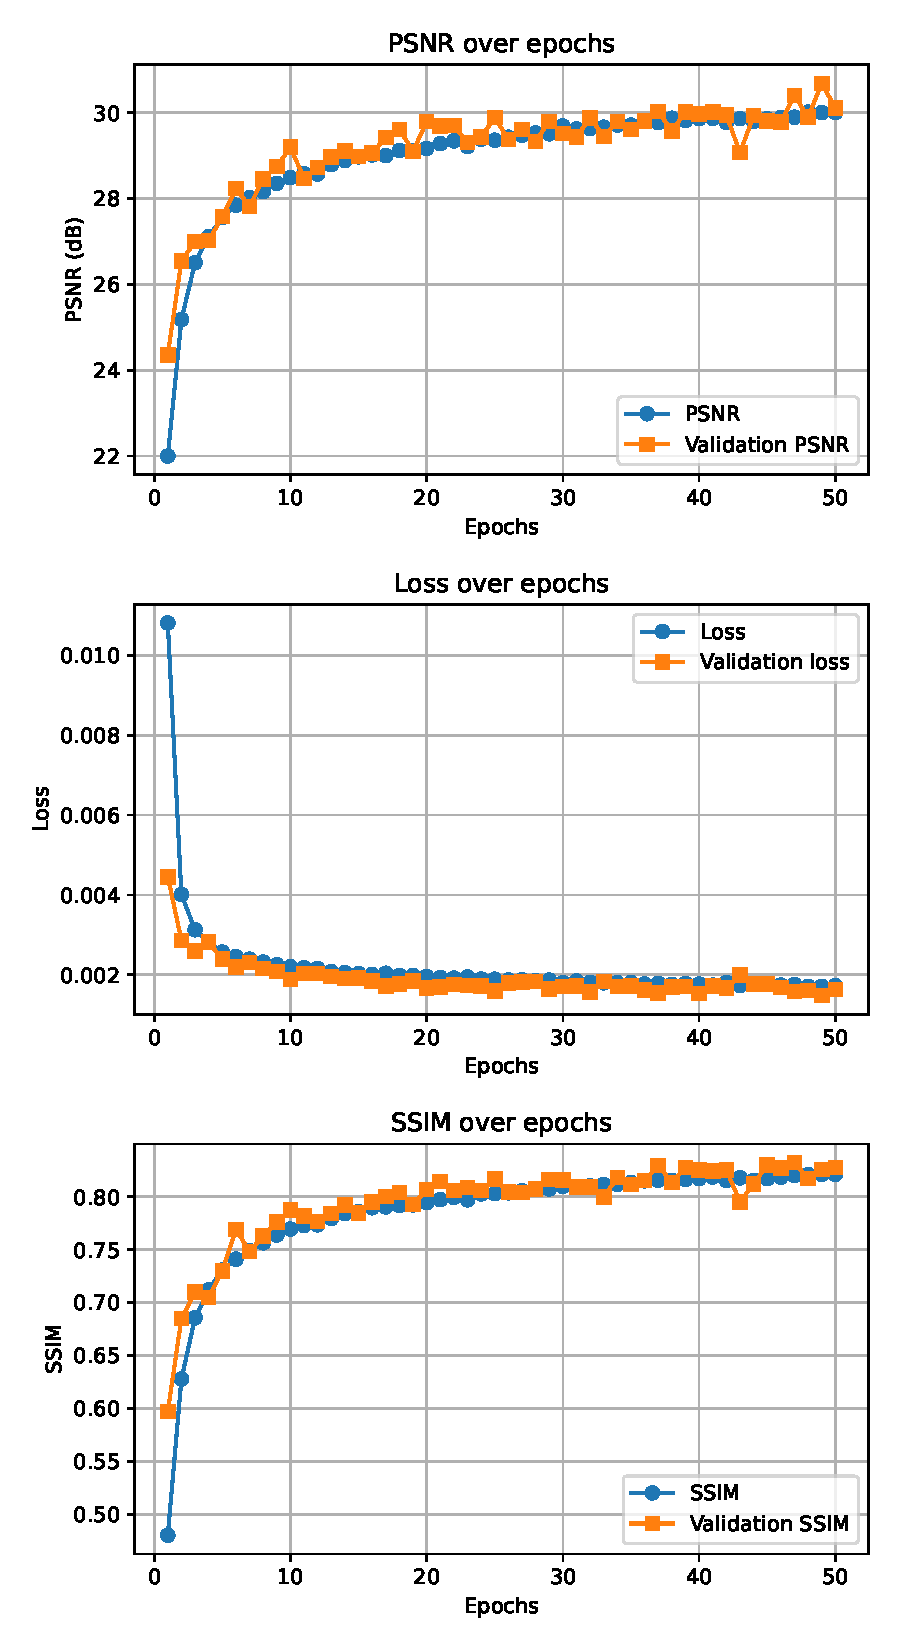
\includegraphics[height=0.9\textheight]{img/ch6/supervised/psnr_loss_unet.pdf}
        \caption{U-Net}
        \label{fig:denoising-exp1-curves-unet}
    \end{subfigure}
    \caption{PSNR, loss, and SSIM curves for the (a) Irfan and (b) U-Net models for Experiment 1.}
    \label{fig:denoising-exp1-curves}
\end{figure}


%%%%%
\newpage
\subsection{Experiment 2}

\vfill

\begin{figure}[htbp]
    \centering
    \begin{subfigure}{\textwidth}
        \centering
        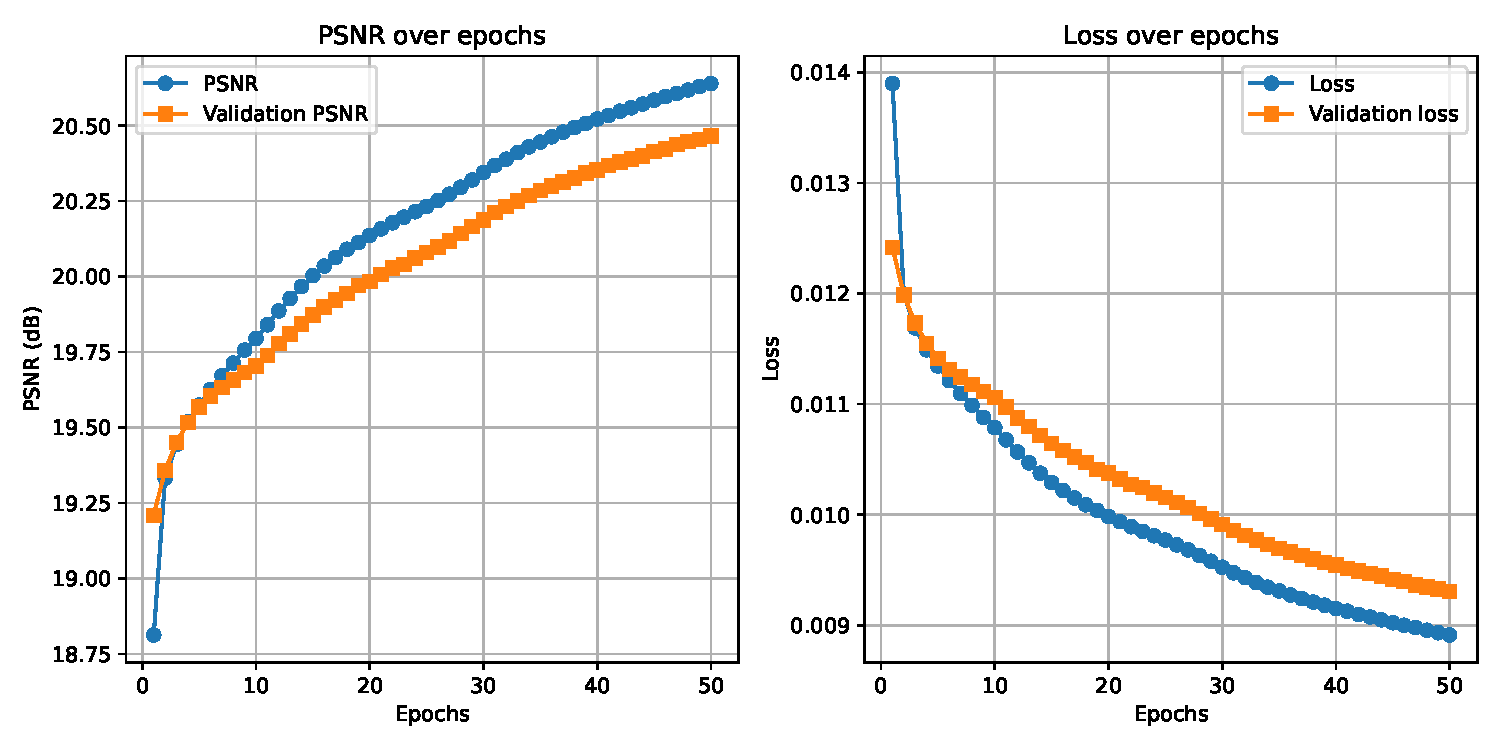
\includegraphics[width=\textwidth]{img/ch6/in_eq_out/irfan/psnr_loss_curves.pdf}
        \caption{PSNR and loss curves for the Irfan model, trained over 50 epochs.}
        \label{fig:denoising-exp2-curves-irfan}
    \end{subfigure}
    
    \vspace{0.5cm}
    
    \begin{subfigure}{\textwidth}
        \centering
        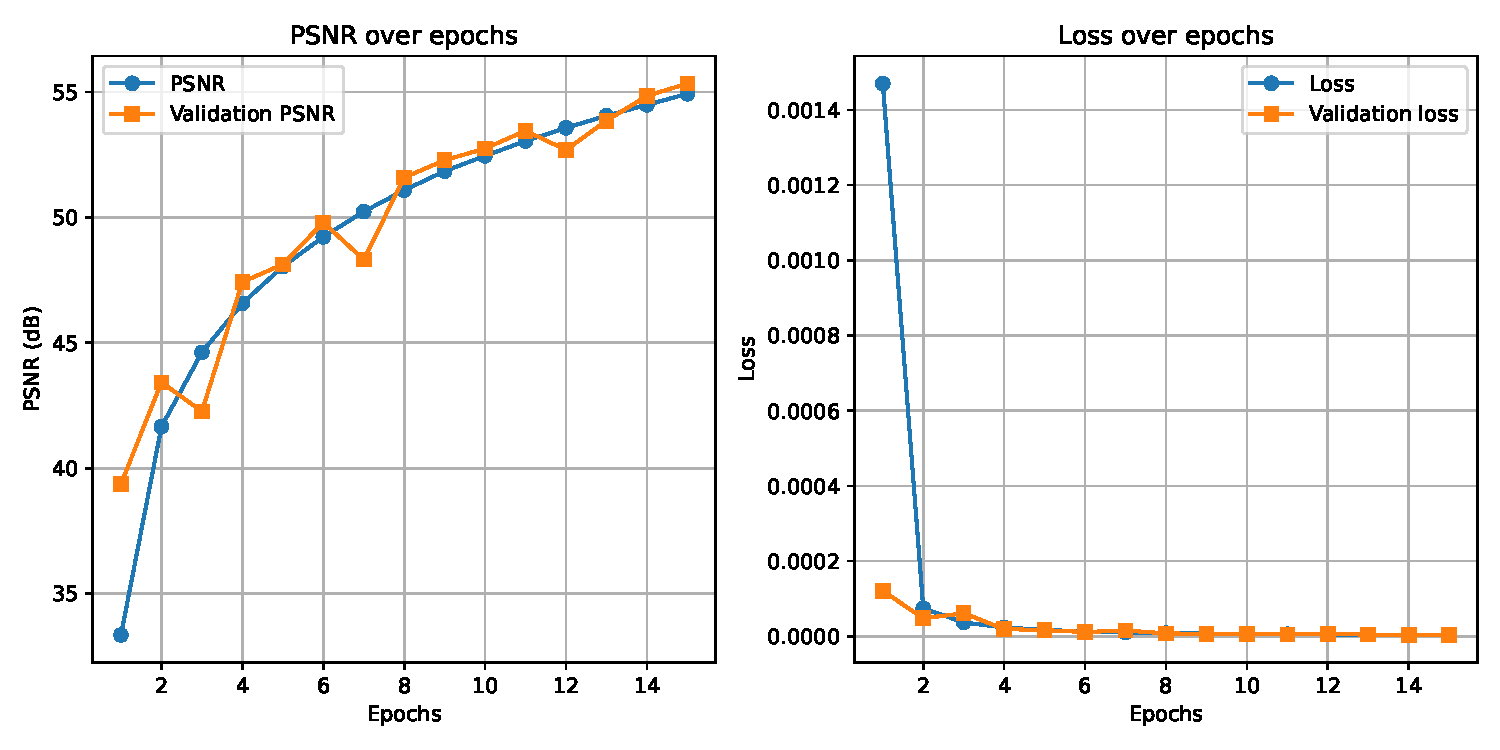
\includegraphics[width=\textwidth]{img/ch6/in_eq_out/unet/psnr_loss_curves.pdf}
        \caption{PSNR and loss curves for the U-Net model, trained over 15 epochs due to time constraints.}
        \label{fig:denoising-exp2-curves-unet}
    \end{subfigure}
    \caption{PSNR and loss curves for the (a) Irfan and (b) U-Net models for Experiment 2.}
    \label{fig:denoising-exp2-curves}
\end{figure}

\vfill

%%%%%
\newpage
\subsection{Experiment 3}
\vfill
\begin{figure}[htbp]
    \centering
    \begin{subfigure}{\textwidth}
        \centering
        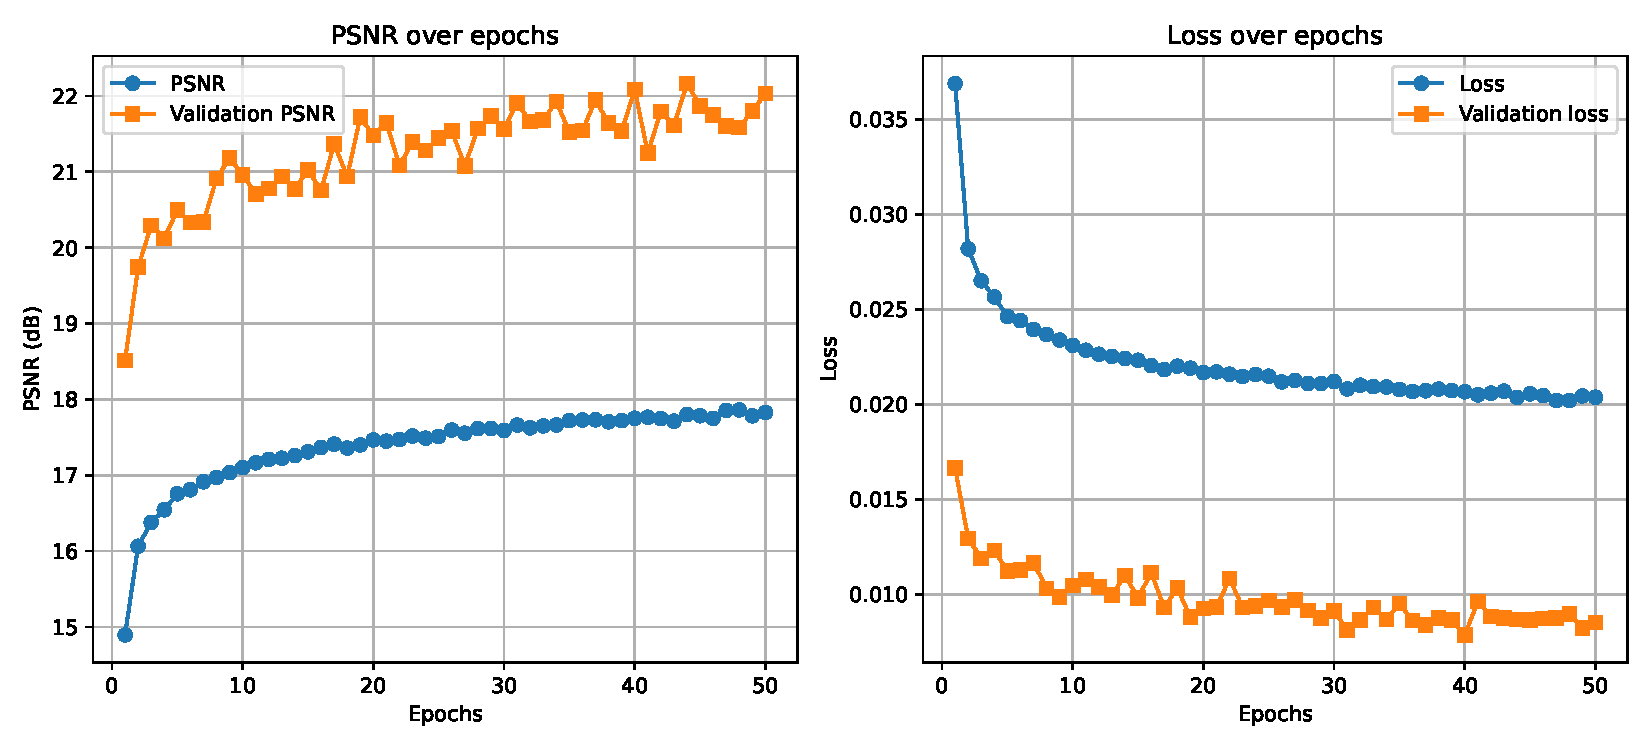
\includegraphics[width=\textwidth]{img/ch6/n2n_imagenet/psnr_loss_irfan.pdf}
        \caption{Irfan}
        \label{fig:denoising-exp3-curves-irfan}
    \end{subfigure}
    
    \vspace{0.5cm}
    
    \begin{subfigure}{\textwidth}
        \centering
        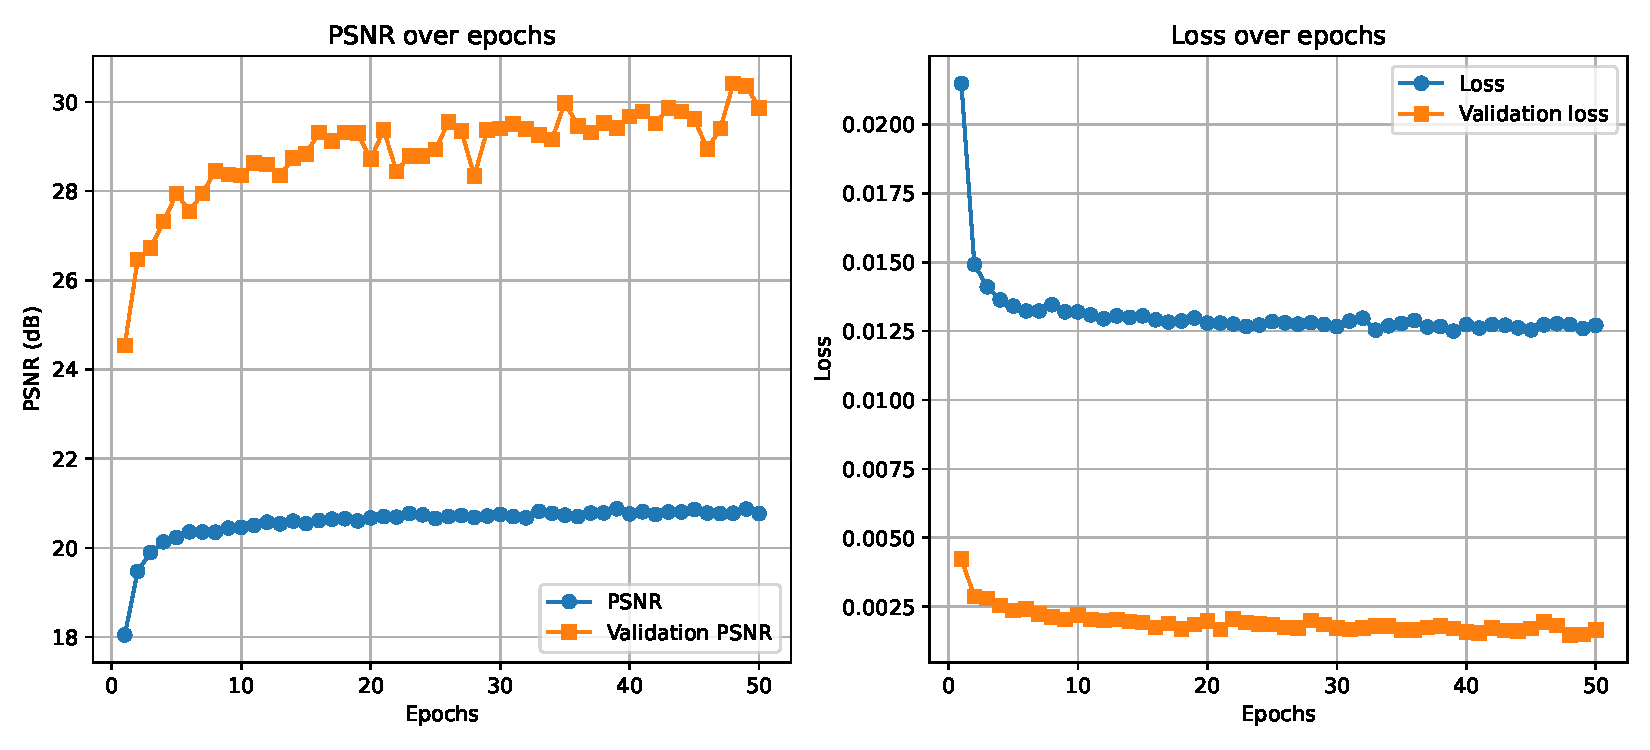
\includegraphics[width=\textwidth]{img/ch6/n2n_imagenet/psnr_loss_unet.pdf}
        \caption{U-Net}
        \label{fig:denoising-exp3-curves-unet}
    \end{subfigure}
    \caption{PSNR and loss curves for our recreation of the Noise2Noise paper \cite{lehtinen_noise2noise_2018}. The denoising approach was evaluated on both (a) Irfan, a basic convolutional encoder-decoder structure, and (b) U-Net, a state-of-the-art machine learning architecture.}
    \label{fig:denoising-exp3-curves}
\end{figure}

\vfill



